\documentclass[a4paper,11pt]{article}
\usepackage[utf8]{inputenc}
\usepackage[ngerman]{babel}
\usepackage{geometry}
\usepackage{graphicx}
\usepackage{amsmath}
\usepackage{hyperref}
\usepackage{enumitem}

\geometry{a4paper, top=2cm, bottom=2cm, left=2cm, right=2cm}	

\usepackage{xcolor}
\definecolor{ohm_red}{RGB}{192,0,0}


\usepackage{fancyhdr}


\usepackage{titling}
\pretitle{\begin{flushleft}\LARGE}
\posttitle{\end{flushleft}}
\preauthor{\begin{flushleft}\large}
\postauthor{\end{flushleft}}

\setlength{\parindent}{0pt}



\pretitle{\begin{flushleft}\huge\textbf{\textcolor{ohm_red}}}
\posttitle{\end{flushleft}}

\pretitle{\begin{flushleft}\huge\textbf{\textcolor{ohm_red}}\rule{\linewidth}{0.4mm}\\}
\posttitle{\\\rule{\linewidth}{0.4mm}\end{flushleft}}
\title{\textcolor{ohm_red}{Visuelle Navigation mit einer Drohne}}

\date{}


\usepackage{enumitem}
\setlist{nosep}

\pagestyle{fancy}
\renewcommand{\headrulewidth}{0pt}
\fancyhead[L]{
\includegraphics[height=2.0cm]{img/logo_autonohm.png}}
\fancyhead[R]{veröffentlicht am \today}


\usepackage{sidecap}

\sidecaptionvpos{figure}{c}


\begin{document}

\maketitle
\thispagestyle{fancy}

\vspace*{-3cm}
\begin{figure}[h!]
    \centering
    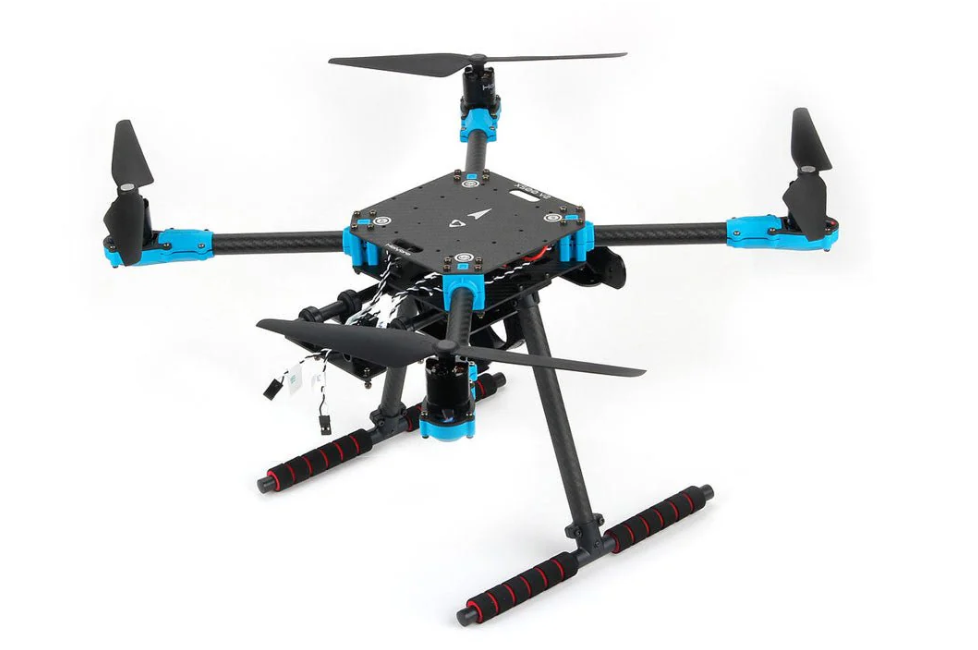
\includegraphics[height=4cm]{img/holybro_x500.png}
    % \caption{Example Image}
    % \label{fig:example}
\end{figure}


Im Rahmen des neu geschaffenen Ohm Innovation Centers (OIC) entsteht auch Europas größte Drohnenhalle für die die angewandte Forschung: 
In einem ersten Schritt soll eine Drohne vom Typ Holybro X500, die mit einem Pixhawk 6 Autopiloten ausgestattet ist, 
selbstständig vorher definierte optische Markierungen (Aruco-Marker) im Raum erkennen und anfliegen. Die Drohne soll dabei mittels ROS (Robot Operating System) gesteuert werden. 

Das Ziel ist es, die Drohne so zu steuern, dass sie die Marker im Raum erkennt und anfliegt. 
Die Drohne soll dabei so navigieren, dass sie die Marker aus verschiedenen Perspektiven erkennen kann. 
In einem ersten Schritt soll die Drohne hierbei eine gleichbleibende Höhe halten und sich nur in der Ebene bewegen. In einem zweiten Schritt soll die Drohne auch die Höhe variieren können um Maker in unterschiedlichen Höhen anfliegen zu können. 

\section*{Arbeitspakete}
\begin{itemize}[leftmargin=0.5cm]
    \item Einarbeitung in die Steuerung der Drohne mittels ROS
    \item Auswahl und Integration einer Kamera an der Drohne
    \item Implementierung oder Parametrierung eines Marker-Erkennung
    \item Test der visuellen Navigation 
\end{itemize}

\section*{Voraussetzungen}
\begin{itemize}[leftmargin=0.5cm]
    \item Grundkenntnisse in ROS 
    \item Grundkenntnisse in einer höheren Programmiersprache (z.B. Python, C++)
    \item Grundkenntnisse in der Bildverarbeitung
\end{itemize}

\vspace{0.5cm}
Das Thema kann nach Abstimmung als Bachelor- oder Masterarbeit bearbeitet werden, sowie als Projektarbeit. 


\vfill
\textcolor{ohm_red}{\rule{\linewidth}{0.4mm}}
\textbf{\textcolor{ohm_red}{Labor für mobile Robotik}} \\
\begin{tabular}{@{}ll}
\textbf{Betreuer:} & Prof. Dr. Christian Pfitzner \\
\textbf{E-Mail:}   & \href{mailto:christian.pfitzner@th-nuernberg.de}{christian.pfitzner@th-nuernberg.de} \\
\end{tabular}

\end{document}